\documentclass[output=paper]{langsci/langscibook} 
\author{%
Fabio Alves \affiliation{UFMG, \href{mailto:fabio-alves@ufmg.br}fabio-alves@ufmg.br}
\and
Karina Sarto Szpak \affiliation{UFMG, \href{mailto:kszpak@ufmg.br}kszpak@ufmg.br}
\and
José Luiz Gonçalves \affiliation{UFOP, \href{mailto:zeluizvr@ichs.ufop.br}zeluizvr@ichs.ufop.br}
\and
Kyoko Sekino \affiliation{UFMG, \href{mailto:kyokosekino@ufmg.br}kyokosekino@ufmg.br}
\and
Marceli Aquino \affiliation{UFMG, \href{mailto:marceliaquinoufmg@gmail.com}marceliaquinoufmg@gmail.com}
\and
Rodrigo Araújo de Castro \affiliation{UFMG, \href{mailto:roacastro87@yahoo.com.br}roacastro87@yahoo.com.br}
\and
Arlene Koglin \affiliation{UFMG, \href{mailto:arlenekoglin@yahoo.com.br}arlenekoglin@yahoo.com.br}
\and
Norma B. de Lima Fonseca \affiliation{UFMG, \href{mailto:normafonseca@ufmg.br}normafonseca@ufmg.br}
\lastand
Bartolomé Mesa-Lao \affiliation{CBS, \href{mailto:Bm.ibc@cbs.dk}Bm.ibc@cbs.dk}
 }
% \sectionDOI{} %will be filled in at production

\epigram{Change epigram in chapters/01.tex or remove it there }

\abstract{This paper presents the results of an experimental study that investigates the influence of cognitive effort on post-editing tasks from a relevance-theoretic perspective \citep{Wilson2011}. Using two short scientific texts, we compare post-editing processes in two different machine translation web-based workbenches, namely interactive machine translation (IMT) and standard, non-interactive machine translation (MT). The relevance-theoretic concepts of conceptual and procedural encodings \citep{Wilson2011} and the methodology developed by Alves and Gonçalves (2013) to assess cognitive processes in the course of translation tasks are used as the framework for data analysis. Sixteen professional translators performed interactive and non-interactive post-editing tasks in random order, having their processes recorded with the aid of a Tobii T60 eye tracker. Data were collected with the CASMACAT workbench and results pointed to the following conclusions:  (1) as it has been found in human translation (Alves and Gonçalves 2013), the percentage of edits related to procedural encoding is significantly higher than that related to conceptual encoding; (2) interactive post-editing requires less cognitive effort, as shown by the average and median fixation duration which was statistically lower when using the interactive system. As a way of conclusion, the paper reflects on these results and their implications for the development of interactive machine translation platforms for post-editing.
}
\title{Investigating Cognitive Effort in Post-editing: {A} relevance-theoretical approach}
\maketitle
\begin{document}





\section{Introduction}

It has been widely acknowledged that the aim of machine translation is to produce high-quality translation as well as speeding up translation tasks and enhancing the cost-effectiveness of this process. In order to meet the increasing demand for translations, machine-translation technology has been largely adopted by language service providers worldwide, although human translators are still required to post-edit machine-translated outputs (De Almeida 2013, 17). 


Actually, to achieve high-quality products, there is a need for professional human interaction either before or after the machine has processed the data (O´Brien 2004, 3). The intervention before the machine processes is called \textit{pre-editing} and it occurs at the source-language level. The main objective of pre-editing is to reduce time and effort for post-editing by implementing a number of strategies such as text manipulation. The afterwards intervention is called \textit{post-editing} and it occurs at the target-language level to correct possible errors in the MT output (Mesa-Lao 2013). 



In general, post-editing (henceforth PEd, to be differentiated from the procedural encoding acronym [PE] used throughout this paper) consists in correcting or editing texts that have been translated from a source language into a target language by a machine translation system. A useful definition can be found in \citet{Somers2001}, who also gives a description of usefulness and importance of the PEd process to achieve an understandable text from a machine translation output: 


\begin{quote}
As automated translation still has many limitations even nowadays, the corrections made by human linguists remain indispensable to make machine-translated texts more understandable and accessible to readers. (Somers 2001, 138)
\end{quote}


According to Krings, who introduces one of the most extensive works on PEd research, “the question of post-editing effort is the key issue in the evaluation of the practicality of machine translation systems” (2001, 178). He proposes that PEd effort can be measured on three levels: temporal, technical and cognitive. Temporal effort refers to the time taken to post-edit a particular text; technical effort refers to deletions, insertions and text re-ordering; cognitive effort deals with the extent and type of cognitive processes that the translator needs to apply on a machine translation output, i.e., the amount of effort expended in a PEd task (O´Brien 2006). In this work we focus our attention on the third level proposed by Krings, that is, cognitive effort seen from a relevance-theoretic perspective (Sperber and Wilson 1986/1995), wherein the concepts of conceptual, procedural and hybrid encodings underpin the framework for data analysis. These concepts will be further explored in the next section.



Relevance Theory (RT henceforth) postulates that human cognition is guided by relevance, i.e., essentially seeking information that is relevant for obtaining as many cognitive effects as possible. In other words, RT is based on the premise that our cognition seeks to achieve the greatest cognitive effects through the minimum necessary processing effort. According to Wilson (2011, 72), the human cognitive system tends to “follow a path of least effort in looking for implications; test interpretations in order of accessibility, and stop when your expectations of relevance are satisfied”. 



In this sense, post-editing tasks seem to fit RT assumptions since, according to Loffler-Laurian (1984; 1996), one of the main characteristics of PEd would be the quicker turnaround (in comparison to human translation from scratch), and its focus on corrections that are essential and relevant. In accordance with Loffler-Laurian’s work, in the past few years there has been increasing evidence for productivity gains when professional translators have post-edited machine translation output. Empirical research has demonstrated that PEd can lead to higher productivity. A significant number of studies have compared PEd against translation from scratch. Results from these studies indicate that PEd processes can be very efficient, showing productivity gains of 80\% (Plitt and Masselot 2010; Skadi\c{n}š et al. 2011; Pouliquen et al. 2011; Federico et al. 2012). 



Even with the significant research about the process of post-editing tasks -{}- e.g. Guerberof \citet{Arenas2012}, O’Brien (2006; 2009), \citet{Depraetere2010}, Plitt and \citet{Masselot2010}, \citet{SousaEtAl2011}, Specia (2009; 2011) -{}- there is more to know about its usefulness and the influence on the translators’ decision-making processes. 



Considering these studies, this paper aims at contributing to PEd research by investigating processing effort, drawing on the concepts of conceptual, procedural and hybrid encodings over two post-editing tasks performed with the aid of the CASMACAT workbench, a statistical machine translation system, used in conjunction with a Tobii T60 eye tracker.



To that end, this article is divided into five sections, including this Introduction. In section 2, we outline the theoretical underpinnings, with special attention dedicated to the concepts of conceptual, procedural and hybrid encodings (Moeschler 1998; Wilson 2011; Alves and Gonçalves 2013). In section 3, we discuss our methodological framework. In section 4, we turn to the statistical analysis, explaining the main distinction between effort spent on interactive and non-interactive post-editing tasks. Finally, we end the article with discussions and concluding remarks in section 5.


\section{Theoretical underpinnings}

This section describes and discusses some concepts from Relevance Theory (Sperber and Wilson 1986/1995) and their application to the problems concerning cognitive effort in post-editing experimental tasks. 


Sperber and Wilson’s \textit{Relevance: communication and cognition} (1986/1995) outlines a very productive and powerful framework for describing and explaining human communicative interactions from two important scientific domains: pragmatics and cognitive studies. While postulating the principle of relevance, the authors introduced a consistent way of integrating these two domains and shed new light on issues concerning language processing as the core of human communicative interactions. They revisited and reformulated key concepts such as context, mutual knowledge, cooperation, code, inference, and representation, among others, into a very coherent and parsimonious framework.



In this section, we will present some concepts from Relevance Theory required to develop the analyses and discussions on the problems we have focused on.


\subsection{The principle of relevance}

RT postulates its principle as a mechanism that produces a balance between processing effort and cognitive effects: “[…] in any given inferential process, the human being’s cognitive environment searches for the generation of the maximum cognitive effects possible while spending the minimum processing effort necessary to achieve this end” (Alves and Gonçalves 2013, 109). Therefore, the principle of relevance regulates effort and effect relations in inferential processing in order to enhance human beings’ cognitive environments. Thus, this guarantees one’s cognitive adaptation to one’s physical and social environments. In short, it is a kind of economic and adaptive principle.


For instance, if a piece of inferential processing demands too much effort, and in turn gives insufficient or very few relevant results (or cognitive effects), it will probably be interrupted or even abandoned, i.e., the person will tend to give up going ahead with that specific piece of processing. On the other hand, if inferential processing tends to achieve a lot of effects, the human cognitive system will indicate when the quantity and quality of those effects are enough/adequate, determining that it has reached optimal relevance, which is a kind of cognitive “satisfaction”. Therefore, this principle prevents the cognitive system from spending unproductive or unnecessary processing effort.



More specifically, RT accounts for the unfolding of human inferential processes through the following sequence:


  
\begin{figure}
 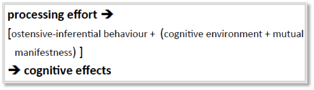
\includegraphics[width=\textwidth]{figures/Sarto1.png}
 \caption{The relevance-theoretic comprehension procedure (Adapted from Alves and Gonçalves (2003, 6)}
 \label{fig:1}
\end{figure} 



Figure \ref{fig:1} schematically summarizes which aspects are required for a certain amount of processing effort to generate a number of cognitive effects. Whenever the ostensive-inferential condition is achieved, inferential communication is about to take place, that is to say, when two interacting individuals (a communicator and a hearer) share a certain level of cognitive representations (i.e., when they reach some level of mutual manifestness) in their cognitive environments, they are ready to communicate. A communicative process is expected to generate as many cognitive effects as possible in the hearer’s cognitive environment. This presumption of relevance (generating the maximum of effects possible with the minimum of effort necessary) is another requirement for communication to take place. Therefore, in ostensive-inferential communication, humans try to avoid unnecessary processing effort when there is no benefit in terms of cognitive effects.



Next, we will discuss how this principle can be productive for translation-related issues.


\subsection{Interpretive resemblance}

When applied to translation, the principle of relevance is expanded to take into account the concept of \textit{interpretive resemblance}. This concept has been developed in the RT framework from the notion of \textit{interpretive use} of mental representations, a second-order level of representations, as opposed to \textit{descriptive use }of mental representations, a first-order level of representations. In short, \textit{descriptive use }establishes a correlation between real or fictional world phenomena/objects and mental representations, while \textit{interpretive use} correlates pairs of mental representations.\\

For instance, when someone says \\

"Mary is coming to the party."\\

the hearer in this situation will build up in her cognitive environment a representation of an event or state of affairs in the real world or in an imaginary world. In this example, there is a case of \textit{descriptive use} of language, connecting a mental representation to an event (whether real or not).\\

On the other hand, if someone says\\

"I don’t believe Mary is coming to the party."\\

the hearer, in this second situation, will have not only to represent a state of affairs or event from the external world in her cognitive environment, but also that it is represented as not true in the speaker’s cognitive environment. Here, there is a case of \textit{interpretive use}, i.e., the hearer creates a second order mental representation aiming at resembling the speaker’s mental representation behind that utterance. 


Building on this notion of \textit{interpretive use}, Gutt (1991/2000) defined translation as the search for \textit{interpretive resemblance }between corresponding utterances, one in the source language and the other in the target language. Gonçalves (2003) expanded the focus of that definition, applying it to the concept of translation unit (TU) as the entity to be individually interpreted, transferred and compared in the course of the translation process. According to Gonçalves (2003), this process is aimed at maximizing \textit{interpretive resemblance }between a source-text translation unit and its target-text counterpart. This \textit{interpretive resemblance}, in line with the principle of relevance, determines that the production of contextual or cognitive effects from the interpretation of the source-text translation unit should overlap, as much as possible, with those effects found in the production/interpretation of the counterpart target-text translation unit. The effects from both source and target language TUs are represented by the respective sets of explicatures (the explicit semantic content of a linguistic input) and implicatures (the less explicit and progressively implicit content, i.e., the inferred implications of that input).



To build up \textit{interpretive resemblance} in translation, the translator is expected to \textit{meta-represent} his/her audience’s cognitive environment. Meta-representations are higher order representations that allow the communicator, among other things, to simulate mentally his/her audience’s inferential context (as well as that of the source text author and source text audience) in order to achieve the most adequate cognitive effects through the production of appropriate stimuli in target language.  



In the process of post-editing, post-editors are guided by the meta-representation that the final product  has to be good enough for the purposes agreed upon with the client (either a fast, light or a full, human-quality post-edited translation) necessarily spending less time than translating from scratch (\textit{cf. }Carl et al 2014; Sanchis-Trilles et al 2014). As it will be discussed in section 2.4, it is very important that post-editors bear in mind the crucial relation between time (effort) and quality (effects) for the success of post-editing tasks, reducing time (and eventually processing effort) to a minimum possible and increasing quality (related to cognitive/contextual effects) to the maximum required for the PEd modality in focus or almost as good as a human professional translation.



Therefore, especially in fast, light PEd, translation acceptability by the target audience will be more flexible. Considering that one of the goals in PEd in this modality is to achieve a good enough target text in the shortest time possible, processing effort commonly spent on stylistic refining will tend to be avoided or reduced to a minimum since the main goal in that particular task modality is, in most cases, to offer, as soon as possible, a reasonably understandable product to its audience. 



While translating from scratch, translators tend to generate a number of implicatures for a certain problematic translation unit. As Alves and Gonçalves (2007) pointed out, the more expert the translator is, the greater the number of implicatures s/he will be able to generate for a problematic unit in order to choose the one that will best suit a relevance-oriented processing in his/her audience’s cognitive environment – a textual input that may generate the maximum (and the most precise) cognitive effects possible with the minimum processing effort necessary to accomplish the task. 



In PEd, however, due to higher time pressure demands, the translator/post-editor is expected to save time and cognitive effort as the machine translation (MT) system generates a first version of the target text. Thus, still following the principle of relevance, s/he will try to find a good enough solution (always considering the modality of PEd agreed upon for the task – fast or full), calculating its effects on the audience’s cognitive environment and, then, accepting integrally or partially the raw MT output. More specifically, while post-editing a machine translation output with the help of an interactive system (IMT), the post-editor will be offered some optional solutions for a specific problem in case he decides to change something in a translation unit. These solutions offered by the IMT system will change the post-editors’ reading purpose since, from an initial change, all the rest of the output is automatically changed, remaining to the post-editor the decision of either reading for revision or  for post-editing. 



In this regard, Jakobsen and \citet{Jensen2008} investigated the effects of the type of task (reading for understanding, for translating, for sight translation, and for written translation) on eye movements and concluded that the reading purpose had a clear effect on eye movements and on gaze time. Thereby, interactive systems are expected to show an effect on eye movements related to post-editing processes by reducing the cognitive processing effort demanded during the output revision, as it will be postulated in one of our hypotheses and discussed in section 4.


\subsection{Conceptual and procedural encodings}

As we have shown in the preceding subsections, the main focus of RT is on inferential processes, as they are decisive for an individual’s cognitive improvement and adaptation to his/her physical and social environment. However, some studies building on RT (\textit{e.g. }Moeschler 1998; Blakemore 2002; Wilson 2011; Alves and Gonçalves 2003; 2013) have focused on encoding/decoding as the initial, triggering (and therefore essential) stage of the cognitive processing for verbal communication. \citet{Moeschler1998} postulates the distinction between conceptual and procedural encodings.


In Relevance Theory, a major distinction is made between two types of linguistically encoded information: conceptual information and procedural information (Wilson \& Sperber 1993). The conceptual/procedural distinction is motivated both linguistically and cognitively.



1. Conceptual information is mainly encoded within lexical categories (Noun, Verb, Adjective), that is, categories which define open lexical classes. Procedural information is encoded within non-lexical categories (negation, tenses, determiners, connectives, certain adverbials), that is, categories which define non-open morphological classes. Thus the conceptual/procedural distinction covers mainly the distinction between lexical and non-lexical categories.



2. The cognitive motivation for the procedural/conceptual distinction is the following: conceptual information is information through which mental representations are accessible, whereas procedural information encodes instructions relative to how mental representations must be processed. (Moeschler 1998, 1)



On the one hand, as conceptual encodings refer to, say, more concrete entities, with extra-linguistic references, as nouns, adjectives, verbs, mainly, they are subject to conscious access. On the other hand, procedural encodings, encompassing morph-syntactical rules and restrictions on language structure, are not usually amenable to conscious processing, except indirectly, through meta-cognitive reflection. 



As Alves, Gonçalves and \citet{Szpak2014} explain, the function of conceptual expressions (i.e., open lexical categories, such as nouns, adjectives and verbs) is to convey conceptual meaning which is propositionally extendable and contributes to expanding the inferential processing of an utterance whereas the function of procedural expressions is to activate domain-specific cognitive procedures (i.e., morph-syntactic constraints in utterance processing) and contributes to constraining the inferential processing of these same utterances. Relevance Theory assumes that the conceptual-procedural distinction guides inferential processing. (Alves, Gonçalves and Szpak 2014, 155)  



Besides conceptual and procedural encodings, Alves and Gonçalves (2013), drawing on Wilson’s (2011) arguments, postulated a third category of encoding for a lexical item – the hybrid encoders (HE). These hybrid encodings are found in lexical items including both encoding functions, which encompass most words since exclusively conceptually encoded items are rather the exception than the rule in terms of linguistic encoding.



The studies of \citet{Alves2007} and Alves and Gonçalves (2003) have corroborated the principle of relevance while showing a relation between processing effort and cognitive effects in translation. The authors have also shown that there is an important distinction between the role of conceptual and procedural encodings.  However, those were small-scale studies and only offered qualitative results. Alves and Gonçalves (2013) used a larger sample to build on the previous relevance-theoretic findings and corroborated them by means of statistical analyses. Using key-logged data to map instances of conceptual and procedural encodings onto micro/macro translation units (Alves and Vale 2009; 2011), Alves and Gonçalves (2013) concluded from their results that problems related to procedural encodings demand more processing effort both in direct and inverse translation tasks.


\subsection{Post-editing, relevance and encoding}

As we mentioned above, post-editing aims at offering an acceptable and intelligible target text for a certain audience in a specific context within a significantly shorter period of time than that spent in a human translation. And as in any translation process, the aim is maximizing interpretive resemblance between source and target texts. Thus, in PEd as well, a post-editor seeks for a product (a post-edited target text) that will optimally resemble the source text, or that will resemble it in relevant aspects. 


In this respect, depending on the type of post-editing agreed between client and translator, there will be more or less acceptability and tolerance for minor formal and stylistic inaccuracies in the post-edited text. In Relevance Theory terms, the target text receptor will be more inclined and ready to overcome some small imperfections, accepting a certain increase in the processing effort to achieve the cognitive effects that will lead him/her to optimal interpretive resemblance. In this case, the reader accepts that a post-edited product demands slightly more effort to be processed but supposedly results in the expected (and approximately the same amount of) effects as in human translation – reader and client accept this state of affairs since the deadline is usually much shorter and the cost significantly cheaper for the product. Therefore, in PEd “the demand of faster and cheaper translations increases” (Aziz, Koponen and Specia 2014, 171). It is important to highlight that, according to the principle of relevance, there are limits for this acceptability – the cognitive effort demanded from the audience may not surpass a certain limit and the effects are expected to optimally (or minimally in relevant aspects) resemble those in the source text.



Taking into account Alves and Gonçalves’s (2013) results, that procedural encoding (PE) edits are more prevalent than conceptual encodings (CE) edits in human translation, and that machine translation systems have been developed to facilitate human translation tasks, it is important to ask if this prevalence will be kept or modified in PEd.



Some highly optimistic approaches to PEd say so. \citet{GreenEtAl2013}, for instance, report that the use of basic post-editing tools by bilingual human translators improve translation quality in comparison to texts produced by bilingual human translators working without assistance from machine translation and post-editing tools. Actually, some sophisticated interactive interfaces, like translation memories (TM), machine translation (MT), computer assisted MT, statistical MT (SMT), interactive translation prediction (ITP) approach (Langlais and Lapalme, 2002; Casacuberta et al. 2009; Barrachina et al. 2009), online learning approach (Ortiz-Martínez et al., 2010; 2011), active learning approach (González-Rubio and Casacuberta 2014), and multitask learning approach (C. de Souza et al, 2014), may also provide benefit, especially with regard to post-editors’ productivity, i.e., reduction of time, cost and processing effort.


\subsection{Hypotheses}

\begin{enumerate}
\item In IMT condition, there will be less instances of editing events (total, CE, PE) than in MT condition, since the interactive system is expected to provide more optional and possibly better solutions as soon as the post-editor starts editing a certain unit, thus preventing him/her to proceed with that specific piece of editing.
\item As in Alves and Gonçalves (2013), there will be more instances of procedural than conceptual related edits in PEd, both in MT and IMT condition. We expect that machine translation will most likely solve and/or reduce problems related to conceptual than to procedural encodings, leaving procedural related problems to be solved by post-editing procedures.
\item In IMT condition, the average and median duration of an~eye-fixation~will be shorter than in MT condition, since the interactive system is expected to reduce processing effort when compared to the non-interactive system. Drawing on Jakobson and \citet{Jensen2008}, we expect that in IMT there will be more reading for checking and revising than for writing and editing, that is more frequent in MT.
\item Considering PE and CE edits, as interactive machine translation is expected to reduce cognitive effort, the average fixation duration per edit (CE and PE) will be shorter in the IMT condition than in the MT condition.
\end{enumerate}

Based on these hypotheses, the main goal of this paper is to investigate the impact of conceptual, procedural and hybrid encoding edits over the cognitive effort patterns observed in the interactive and non-interactive post-editing processes by Brazilian professional translators in the English-Portuguese language pair.


\section{Methodological Framework}

This section is divided into two subsections. First, we introduce the experimental design; secondly, we present the methodology for data analysis, giving special attention to the procedures for annotating post-editing process data.   

\subsection{Experimental design}

Sixteen Brazilian translators, with at least five years of professional experience, were asked to post-edit, into Brazilian Portuguese (L1), two source texts in English (L2) about the clinical results of two different pharmacological products, Hycamtin and Protaphane (see Appendix). Before starting the task, participants were instructed through a brief with a detailed description on the procedures.


Data were collected using the CASMACAT workbench (Cognitive Analysis and Statistical Methods for Advanced Computer Aided Translation), a statistical machine translation (SMT) system developed by the CASMACAT project team, in conjunction with a Tobii T60 eye tracker, at the Laboratory for Experimentation in Translation (LETRA) in Brazil. In order to remove the effects of participants’ heterogeneity, a randomized block design, in which the plots form a set of eight replicated 2x2 Latin squares, was used. Thereby, source texts were post-edited in a random order, as well as the type of workbench configuration, non-interactive machine translation (MT) or interactive machine translation (IMT).



According to \citet{AlabauEtAl2013}, in the IMT approach, a fully-fledged machine translation engine is embedded into a post-editing workbench allowing the system to look for alternative translations whenever the human translator corrects the output offered by the SMT. 



For a given source sentence, the SMT system automatically generates an initial translation that is checked and edited by the participant. The SMT system then proposes a new completion considering the correction. These steps are repeated until the whole input sentence has been correctly translated. In this way, the system produces a suitable prediction according to the text that the participant is writing. Figure \ref{fig:2} shows the IMT workbench in which the grey colour represents the suitable prediction, the red dots indicate eye movement paths, the acronym ITP (Interactive Translation Prediction) identifies the type of workbench and T→ (Start Translating) shows the target text in the selected language of interest. The user can also assign a different status to a segment, for instance, TRANSLATED for finished ones or DRAFT for the ones s/he is not yet sure about the translation and wants to review later.



\begin{figure}
 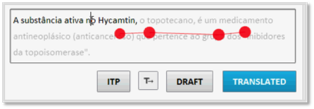
\includegraphics[width=\textwidth]{figures/Sarto2.png}
 \caption{Example of IMT prediction workbench}
 \label{fig:2}
\end{figure} 


In the MT approach, on the other hand, the SMT system produces full target sentences, or portions thereof, which can be accepted or edited by the participant. However, in this case, when an error is corrected, no predictions are offered by the SMT. Figure  \ref{Fig:3} shows the MT workbench, in which the acronym PE stands for post-editing and one can observe that no predictions are offered while the participant is editing the segment.  



  
\begin{figure}
 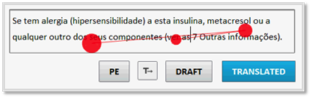
\includegraphics[width=\textwidth]{figures/Sarto3.png}
 \caption{Example of MT workbench}
 \label{fig:3}
\end{figure} 
 

Before the post-editing tasks, participants were asked to fill out a questionnaire in order to collect data about their profiles as professional translators, as well as their previous experience in post-editing. Eye calibration was also performed before the tasks, according to the instructions provided in the Tobii T60 user’s manual.



Building on Alves, Gonçalves and \citet{Szpak2012} and Alves and Gonçalves (2013), the methodology was refined in order to investigate the relevance-theoretic conceptual/procedural distinction in post-editing process. We have thus correlated the edits performed in the text segments to their respective visual activity in selected areas of interest (AOIs). The next subsection presents the methodological steps taken to achieve that end.


\subsection{Procedures for data analysis}

First, for data preparation, each MT and IMT post-editing task was filtered in order to avoid the overlapping of eye-activity data (for detailed information on filtering eye-tracking data, see Alves, Gonçalves and Szpak 2012). Thus, we created a set of scenes containing only eye-tracking data directly related to an individual segment at a given time. In order to clarify this methodological procedure, it is necessary to explain how the SMT system operates.  


The CASMACAT workbench is a web-based CAT tool with an entry point in a web page that the users log into using a personal user name and a password. Once the user has been logged on and selected an assignment, the text opens up in the actual CAT tool. The source text appears in segments on the left and the target text on the right. 



In this study, we worked with 17 segments for the text about Protaphane and 19 segments for the text about Hycamtin. Once the post-editing tasks were randomized, this difference between the number of segments in each text was not a problem in terms of data analysis. Differences in text size and complexity will be explored in other studies on the same data. 



In order to access all the segments provided by the CASMACAT workbench,  participants had to use the scroll bar, which can be a problem when recording gaze activity with the Tobii T-60 eye-tracker, as participants tend to keep their focus of attention on the centre of the screen, causing data overlap, as can be seen in Figure \ref{fig:4}. 


  
\begin{figure}
 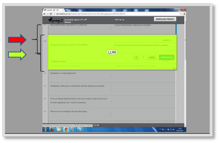
\includegraphics[width=\textwidth]{figures/Sarto4.png}
 \caption{Example of segment data overlap}
 \label{fig:4}
\end{figure} 


On the left, we can observe the area corresponding to the first segment, displayed in red, and, on the right, the second segment displayed in green, with the brackets representing the extent of the visual activity area applied to each segment, where the overlapping is visible. 



Thus, based on Alves, Gonçalves and Szpak’s (2012) methodology, all participants’ data had to be filtered. Using Tobii Studio replay mode, we selected each ST/TT segment and a set of 17 scenes were created for the text about Protaphane and a set of 19 scenes were created for the text about Hycamtin. This can be seen in Figure \ref{fig:5}.  At the bottom of the screen, it is possible to visualize the process time line shown in the selection bar, right under it one can see the scenes created according to the segments provided by the CASMACAT workbench. 


\begin{figure}
 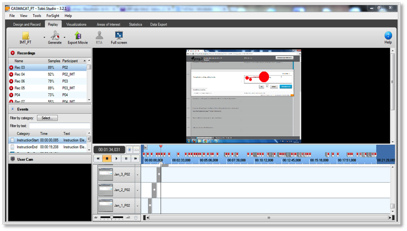
\includegraphics[width=\textwidth]{figures/Sarto5.png}
 \caption{Filtering individual eye-tracking data segment by segment}
 \label{fig:5}
\end{figure} 

As a second step, AOIs were created in order to extract statistically relevant information on gaze activity. Using Tobii Studio 3.2.3, we obtained measures for fixation count and their duration. Drawing on Sjørup (2013, 105), we applied a fixation duration threshold of 180 milliseconds in order to discriminate acceptable data from non-acceptable data. The software generated an Excel file containing data for all participants in both tasks, which serves as the basis for our statistical analyses.



As a third step, in our attempt to map instances of conceptual, procedural and hybrid encodings onto post-editing process data, we had to annotate the editing procedures (deletions, insertions, clause reordering) performed in each textual segment. To that end, the videos recorded while participants performed the post-editing tasks were analysed and a frequency table containing number and type of encodings were created. 



We based our annotation on the categories proposed by Alves and Gonçalves (2013), wherein the total number of conceptual encodings is equivalent to the sum of lexical editing procedures and complex phrasal structure editing procedures \{[l] + [p]\}; the total number of procedural encodings is equal to the sum of a morph-syntactic editing procedures and complex phrasal structure editing procedures \{[m] + [p]\}; and the total number of hybrid encodings is equal to the editing procedures where a lexical item includes both encoding functions [p]. 



Therefore, the editing procedures performed in the complete set of 36 segments were annotated individually with reference to the input offered by the SMT systems.  The data coming from this annotation were correlated to the eye-tracking data, so we could analyse the cognitive effort patterns applied to each type of workbench configuration, (MT) and (IMT). 



Thus, the number of edits on all types of encodings performed in each segment were analysed according to four different types of methodological analyses: i) the number of encoding edits per task, that gives an overall impression of which condition, MT or IMT, demands higher number of  edits related either to conceptual or procedural encoding, ii) the number of eye fixations per condition, that presents the total number of fixations allocated during a post-editing task, iii) fixation duration per condition (MT and IMT), that discusses how cognitively demanding the different post-editing workbench systems are, and iv) average/median fixation duration per condition, that discusses the difference between the two post-editing conditions in terms of cognitive effort.   


\section{Analysis and Discussion}

\subsection{Results }

The results presented in this section are mainly comparisons of the number of edits related to CE, PE and HE encodings and the variables of eye tracking data, such as fixation counts, fixation duration and average/median fixation duration between conditions. Initially, we will present the results of edits on encodings in MT and IMT condition. Next, we will analyse the results regarding visual activity. Finally, we will assess the data to correlate edits and visual activity. 

\subsubsection{Edits in encodings}

The edits related to conceptual, procedural and hybrid encodings were annotated and counted individually as shown in \tabref{tab:1}.


Initially, we characterize our data on encodings in order to make clear the relation between CE, PE and HE.  Before our detailed analysis, we realized that hybrid encodings had an extremely low occurrence, less than 1\% of all edits. Thus, in this study we only analyse edits in CE and PE, distributing HE to CE and PE equally (\textit{cf. }Alves and Gonçalves 2013\textit{)}. The total number of CE and PE is summarized in \tabref{tab:2}.



Looking at overall editing-related results, contrasting the two conditions, that is,  MT vs. IMT, without distinguishing the texts, we found no difference in the total number of edits (\textit{M}= 26.9 for MT and \textit{M}= 33.8 for IMT, \textit{t}(15) = 1.31, \textit{ns}). Likewise, we found no difference in the number of CE edits contrasting MT to IMT (8.2 ${\approx}$ 12.1), neither in PE (18.7 ${\approx}$ 21.2). These results did not corroborate our first hypothesis. 



As for one of our main objectives, we found a significant difference in the total number of edits between CE and PE in MT condition, 8.2 (CE) {\textless} 18.7 (PE),               \textit{t}(15) = -7.38, \textit{p} {\textless} .01, as well as in IMT condition, 12.1 (CE) {\textless} 21.2 (PE ), \textit{t}(15) = -7.21,     \textit{p} {\textless} .00001. Thus, we can confirm our second hypothesis and that the results are in line with those in Alves and Gonçalves (2013) in the investigation of encodings in human translation, revealing that post-editing tasks are also mostly driven by instances of procedural encoding edits, whichever the condition is.

\begin{table}
\begin{tabular}{lllllllllll}
\lsptoprule
\hhline{~----------} &  & {\bfseries     MT} & {\bfseries ~} & {\bfseries ~} & \bfseries ~ & \multicolumn{3}{l}{\bfseries                                IMT} & {\bfseries ~} & \bfseries ~\\
Participants & Condition & Text & CE & PE & HE & Condition & Text & CE & PE & HE\\
P02 & MT & PR & 0 & 7 & 0 & IMT & HY & 9 & 18 & 0\\
P03 & MT & HY & 13 & 20 & 1 & IMT & PR & 3 & 14 & 0\\
P04 & MT & PR & 15 & 35 & 0 & IMT & HY & 31 & 28 & 2\\
P05 & MT & HY & 15 & 34 & 0 & IMT & PR & 9 & 18 & 0\\
P06 & MT & PR & 3 & 13 & 0 & IMT & HY & 9 & 20 & 0\\
P09 & MT & HY & 15 & 26 & 0 & IMT & PR & 11 & 13 & 1\\
P10 & MT & PR & 7 & 8 & 1 & IMT & HY & 12 & 29 & 0\\
P11 & MT & HY & 6 & 15 & 1 & IMT & PR & 2 & 8 & 0\\
P12 & MT & PR & 9 & 15 & 0 & IMT & HY & 9 & 18 & 0\\
P13 & MT & HY & 8 & 15 & 0 & IMT & PR & 2 & 17 & 0\\
P14 & MT & PR & 7 & 17 & 0 & IMT & HY & 13 & 23 & 0\\
P15 & MT & HY & 8 & 19 & 1 & IMT & PR & 6 & 23 & 0\\
P16 & MT & PR & 5 & 11 & 0 & IMT & HY & 19 & 23 & 0\\
P18 & MT & PR & 4 & 11 & 0 & IMT & HY & 25 & 38 & 1\\
P19 & MT & HY & 10 & 31 & 0 & IMT & PR & 7 & 19 & 0\\
P21 & MT & PR & 2 & 18 & 0 & IMT & HY & 22 & 35 & 0\\
\lspbottomrule
\end{tabular}
\caption{Number of edits per participant concerning conceptual, procedural and hybrid encodings in MT and IMT conditions.}
\label{tab:1}
\end{table}

\begin{table}
\begin{tabular}{llllll}
\lsptoprule
{~} & {MT} & ~ & {~} & {IMT} & ~\\
Text & CE & PE & Text & CE & PE\\
PR/HY & 131 & 299 & HY/PR & 193 & 348\\
\lspbottomrule
\end{tabular}
\caption{The total number of edits concerning conceptual and procedural encodings in MT and IMT conditions.}
\label{tab:2}
\end{table}


On the one hand, we have found a proportion of less than 30\% of CE edits against more than 70\% of PE edits in the MT condition. Furthermore, in the IMT condition we have found that CE edits corresponded to more than 30\% of the total number of edits while PE edits accounted for a little less than 70\% of the total number of edits, which indicates a higher proportion for PE against CE, as shown in table 3. 

\begin{table}
\begin{tabular}{lllll}
\lsptoprule
~ & \multicolumn{4}{l}{Texts mixed}\\
Conditions & \multicolumn{2}{l}{MT (16)} & \multicolumn{2}{l}{IMT (16)}\\
Encodings & {CE } & PE & {CE } & PE\\
Total & {91} & 295 & {224} & 392\\
\% & {24\%} & 76\% & {36\%} & 64\%\\
results & \multicolumn{2}{l}{\textit{t}(15) = -7.38} & \multicolumn{2}{l}{\textit{t}(15) = -7.21}\\
~ & \multicolumn{2}{l}{\textit{p} {\textless} .01} & \multicolumn{2}{l}{\textit{p} {\textless} .00001}\\
\lspbottomrule
\end{tabular}
\caption{Reporting the total number of edits of CE and PE in each condition}
\label{tab:3}
\end{table}


These results are in line with those by Alves and Gonçalves (2013), namely 42.5\% of edits related to CE against 57.5\% of edits related to PE in human translation with significant difference. Note that, in both PEd conditions, PE edits were significantly higher than CE edits. From this observation, PE is more edited than CE in PEd, even higher than in human translating, indicating that machine translation systems tend to be more productive when dealing with CE-related items (vocabulary and terminology) than with PE-related items (morph-syntax).  



Having assessed the number of CE- and PE-related edits in MT and IMT conditions, our next step was to verify the cognitive effort spent on these post-editing tasks, thus, we present in the next session the analysis of eye-tracking data.


\subsubsection{Fixation count, fixation duration and the average of fixation duration}

We tested the effect of MT and IMT conditions on variables such as fixation count and fixation duration and observed larger numbers in IMT condition in both fixation count and fixation duration, as shown in Figure \ref{fig:6}. Using the Wilcoxon test, results show a statistically significant difference between these conditions [for all the participants, V = 136, \textit{p} {\textless} .05 (1768.25 (IMT) {\textgreater} 901.56 (MT)].


\begin{figure}
 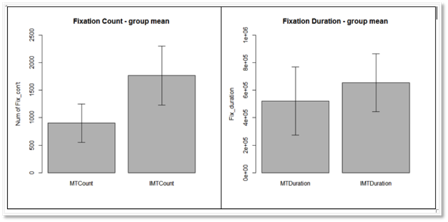
\includegraphics[width=\textwidth]{figures/Sarto6.png}
 \caption{Mean fixation count/duration for MT and IMT: average fixation count (left) an average fixation duration (right)}
 \label{fig:6}
\end{figure} 



Interestingly, when comparing average fixation duration (as it is demonstrated in Figure \ref{fig:7}), the value in MT is greater than in IMT. We tested this difference and observed that the average fixation duration of MT is significantly longer than that in IMT [520684.13 (MT) {\textless} 653518.38 (IMT), \textit{V} = 0, \textit{p} = 0.03]. One may point out that the duration of fixations can vary according to the workbench system in use, consequently, the type of post-editing task. In this sense, we interpret that in terms of fixation data, fixation for reading translation options in IMT condition can be different from that related to processing translation from scratch, as well as that related to non-interactive post-editing, i.e., what may possibly include \textit{from-scratch-type} of problem solving. Under this assumption, we checked the average and the median of MT and IMT fixation durations (\tabref{tab:4}). According to Jakobsen and \citet{Jensen2008}, data concerning to eye movements such as fixation count and fixation duration is sensitive depending on task where reading is predominantly involved. Thus, we find reasonable to postulate that in the IMT condition, fixation duration is more closely related to reading than to \textit{from-scratch-type} of problem solving. 



\begin{figure}
 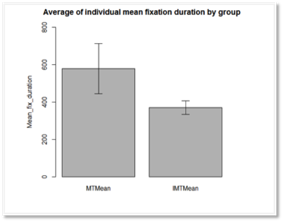
\includegraphics[width=\textwidth]{figures/Sarto7.png}
 \caption{Average fixation duration in MT and IMT (in milliseconds)}
 \label{fig:7}
\end{figure} 


With regard to reading behaviour in IMT workbench, \tabref{tab:4} presents interesting data. Despite the higher number of alternative possibilities and relatively greater number of CE edits performed in this condition, as mentioned earlier, the average fixation duration indicates the effectiveness of the interactive mode, since the effort spent on building up implicatures from the identified encoding problems seems to be reduced by these alternative possibilities offered by the system, generating higher number of fixations with shorter fixations on average. This result may indicate that, in spite of the apparently higher processing effort in IMT condition, due to the higher fixation count and fixation duration observed, there was probably less cognitive effort in this condition. Introducing the median value, that is, the central value of a dataset, it can also characterize the participants’ reading behaviour, buffering pushing up or down effects of some outliers. Recognizing that both the mean and median value in MT is much higher than in IMT, we argue that the median fixation duration in IMT reminds the mean fixation duration of reading text for comprehension presented by Just and Carpenter, 225 ms (1980), as well as presented by Rayner, 200-300 ms (1998). Even though we may need more sophisticated methodology to measure this difference, one of the reasons for these significant difference is that a delay in mean fixation duration probably is an indicator for the kind of cognitive activities involved, other than reading. Therefore, it requires some qualitative explanation about the fundamental difference between the two post-editing conditions, as we will discuss below. 

\begin{table}
\begin{tabular}{lll}
\lsptoprule
\hhline{~--} & Mean & Median\\
MT (Total) & 578,74 & 400\\
IMT (Total) & 369,97 & 266\\
\lspbottomrule
\end{tabular}
\caption{The mean and median for fixation duration in MT and IMT conditions}
\label{tab:4}
\end{table}


This result coherently fits our theoretical framework, as RT assumes that building up explicatures and implicatures from scratch (human translation) or from just one unsatisfactory option offered (MT condition) will be more effortful in terms of cognitive processing in translation than doing this assisted by some more options (IMT condition), as the initial process of articulating CE, PE and HE in the target language translation-unit is anticipated by the system. Therefore, results in \tabref{tab:4} indicate that in MT condition, fixations can more probably be related to reading plus problem-solving processes, while in IMT condition they are much more related to reading and less to problem-solving processes.


\subsubsection{Relating the encoding data and the eye-tracking data.}

Finally, we calculate the average fixation duration per edit, that is, the average fixation duration divided by the average number of edits in each condition in order to observe the contributions that each condition offers. When comparing the two conditions, results present a larger average fixation duration for the MT condition                 (29 (MT) {\textgreater} 11 (IMT), \textit{t}(15) = -4.80, \textit{p} {\textless} .001). Therefore, the fourth hypothesis was confirmed.

\begin{table}
\begin{tabular}{lll}
\lsptoprule
\hhline{~--} & \multicolumn{2}{l}{\bfseries                  Total}\\
\bfseries (ms) & {\bfseries MT(16)} & \bfseries IMT(16)\\
\bfseries Average per unit of edits & {29} & 11\\
\bfseries Results & \multicolumn{2}{l}{\textit{t}(15) = -4.80}\\
& \multicolumn{2}{l}{ \textit{p} {\textless} .001}\\
\hhline{~--}
\lspbottomrule
\end{tabular}
\caption{Average fixation duration per edit by condition}
\label{tab:5}
\end{table}

\subsection{Discussion}

\subsubsection{Considerations about edits on encodings}

Our results suggest that CE and PE-related edits, in both MT and IMT conditions, are in line with the results found by Alves and Gonçalves (2013), the first quantitative study to observe cognitive effort upon edits during human translation underpinned by Relevance Theory (Sperber and Wilson 1986/1995). Accordingly, our current research provides evidence that PE-related edits are still more prevalent than CE-related events in post-editing tasks. This not only corroborates the findings of Alves and Gonçalves (2013), but it also suggests that both MT and IMT conditions are mostly driven by instances of edits related to procedural encodings, which could mean that machine translation outputs seem to help solve more CE-related problems than PE-related ones.



In line with relevance-theoretic assumptions, this evidence also highlights the role of PE-related edits to constrain and control inferential processes in post-editing.  Consequently, we confirm the validity of a relevance-theoretic approach to the analysis of post-editing. We claim that the analysis of the number of edits on three different categories, namely CE, PE and HE, is a promising way to characterize multilingual text production tasks such as translation and post-editing.  



Concerning the difference between MT and IMT in terms of edits, the results did not present any significant difference.  From these results, we understand that, even if the IMT workbench suggests options whenever the post-editor types one or two characters, the options appear somehow in a controlled manner for the post-editors to choose the best one among them. We may argue that two possible and concurrent factors could have caused this result: one is related to the participants’ unfamiliarity with IMT post-editing; the other factor relates to the prediction accuracy of the IMT system.  



In terms of unfamiliarity, Underwood et al. (2014, 553) mention that “post-editors’ performance tended to increase as they became acquainted with the interactive system over an 18-month period”.  Therefore, as our participants were not used to do post-editing in the IMT condition, it seems that the facilitating effect expected to be generated by the interactive condition could not be fully observed in the experiment by means of a reduction in the number of edits and a reduction in the total task time. With regard to the total task time, according to \citet{AlvesEtAl2015}, in a study carried out with the same set of data, participants spent significantly more time when post-editing with interactivity, Wilcoxon signed-rank Test\textit{ z} =10, \textit{p} = 0.001, in other words, 1005161 milliseconds (16min 45s) on MT and 1225812 milliseconds (20min 25s) on IMT. 



In terms of prediction accuracy of the IMT system, we could observe that, in spite of the lack of significant difference in the amount of edits between MT and IMT conditions, as well as the unexpected increase in the IMT condition total task time, a facilitating effect\footnote{ We consider a facilitating effect here only as the main factor in the reduction of the amount of cognitive effort and time spent by the post-editor in the production of the target text first version once it is given by the machine output. Therefore, it is not to be mistaken with semantic priming or schema activation effects observed in similar and closely implemented translation/ post-editing experimental tasks.”} of assisting the post-editor stemming from interactive support could be observed. This finding corroborates the results of Sanches-\citet{TrillesEtAl2014}, in which the authors compare MT and IMT post-editing tasks in terms of total time required to produce the final translation and the amount of key strokes performed during the task. Their results show that, even with little training, IMT post-editing can be as productive as standard MT post-editing in terms of total time required to perform the task, as fewer keystrokes were required in the IMT task. Accordingly, our data also suggest that IMT can be as productive as MT in terms of encoding edits performed in both conditions, revealing that the “ready-to-insert” solutions offered by the IMT system demanded low-processing effort from the post-editors, as we discuss below.


\subsubsection{Considerations about the eye-tracking data}

As O’\citet{Brien2008} points out, interpreting eye-tracking data is not a straightforward task. Our results indicate greater fixation count and fixation duration in IMT post-editing than in MT post-editing. This difference can be interpreted in relation to the number of words automatically offered in the IMT condition: this increase is rather expected, as number of words increase along the task in the IMT. What has drawn our attention is the mean and median value of fixation duration: both values are greater in MT than in IMT tasks. As we have commented earlier, it may be related to a distinctive behaviour in post-editing. Jakobsen and \citet{Jensen2008} identified in their study about reading modalities that mean fixation duration is different, depending on the task type. The Danish participants’ mean fixation duration in reading an English text varied from 205 ms in reading for comprehension to 235 ms in sight translation. Their results confirm that, as far as (standard) human translation is concerned, fixation duration on the source text area is different from fixation duration on the target text area. Additionally, there are also differences between translation students and professional translators in terms of cognitive processing. Building on their results, we postulate that there must be typical reading patterns and different processing effort for MT post-editing and IMT post-editing. If a post-editor expects a type of option to be offered by the IMT system and his/her expectations are met, this may influence his/her behaviour – with less fixation count and less fixation duration. If the IMT system, on the contrary, offers unexpected options against standard language conventions that human translators would be likely to render, this may result in an increase in fixation count and fixation duration.


Rayner’s (1998), when talking about the basic characteristics of eye movements in information processing, reports that mean fixation duration during silent reading is 225ms, while mean fixation duration during typing is 400ms. These fixation durations figure support the assumption that the IMT fixation duration is closely related to a reading process type, once we have found a similar pattern as IMT mean/median fixation duration was 369/266ms, respectively, and MT mean/median fixation duration was 578/400ms, respectively, both representing significant differences between MT and IMT.



Likewise, we assume that the MT mean fixation duration is closely related to a typing mean fixation duration, in which fixations are relatively longer, not only because of cognitive processes of encoding and inferring, but also because of the typing activity occurring more frequently in the MT post-editing task. \citet[396]{Rayner1998} points out that longer fixations during typing is explained by the fact that “the eyes wait in place for the hand to catch up”. \citet{Hvelplund2015} argues that this could very well mean that the eyes focus for longer at the same area not because a particular difficult item is being processed but because the mechanical operation of typing is slower than reading.  



CAT tools, such as MT or IMT systems, can be equipped with a variety of optional windows. O’\citet{Brien2008} reports on the relation between fuzzy matches and eye tracking data with users of SDL TRADOS. She defined one of the AOIs set up in the fuzzy match rate area, which was not frequently visited by participants: the respective mean fixation count is 25.60, while other AOIs’ mean fixation count varies from 79 to 1354. However, the average fixation duration (234.92 ms) on these AOIs is similar to those of other AOIs (between 215 – 255 ms). In this sense, our results concerning the fourth hypothesis make sense in terms of global analysis: the average fixation duration per edits demonstrate post-editors’ greater effort in MT, fixating their eyes longer on fewer number of edits. 



Drawing on relevance-theoretic assumptions, we can also argue that the prevalent number of PE edits over the number of CE edits is an indicator of cognitive effort geared to solving particular problems of a morph-syntactic nature, which often occur in post-editing tasks. \citet{Krings2001} postulates that there are two types of cognitive effort required in post-editing. One is at a lower level, at which post-editors mainly seek linguistic correctness, while the other is at a higher level, involving the post-editor’s engagement with the discourse level.  



Oppositely, CE-related edits can be potentially unlimited when translators become more aware of the ST meaning, as CE belong to open lexical classes \citep{Moeschler1998}. Due to the way it encodes content, CE provides information directly related to mental representations. According to \citet{Alves2001}, one tries to recover the conceptually encoded information conveyed by the sender’s mental representations by means of inferential processes. As the MT condition is a traditional human post-editing task with no assistance other than the machine translation output itself, we believe that post-editors are relatively free to engage in CE-related editing by means of inferential processes, which may indicate a more active commitment in terms of building a coherent target text rather than merely implementing a linguistic correction. Expert post-editors, as far as the quality of machine output and the principle of post-editing are concerned, most likely preserve the MT output, adjusting the target text as it was constructed by MT system, rather than passing their own cultural and stylistic filter. In relevance-theoretic terms, the optimal post-editing tool is required to reduce inferential work in building the options to be considered in the establishment of the interpretative resemblance, not only linguistic correction. 


\section{Concluding Remarks}


In this paper, we have set about measuring and comparing eye movements referring to the number of edits on \emph{conceptual and}{~}\emph{procedural}{~}\emph{encodings }(CE and PE) between two post-editing tasks, namely with and without interactive support (IMT and MT conditions respectively). The main objective was to compare these two modes in order to investigate cognitive effort through the observation of instances of encoding-related edits and the usability and impact of an IMT system in the execution of a post-editing task. 



Four hypotheses were proposed: 



Hypothesis 1 predicted that there would be a lower number of editing events in the IMT condition than in the MT; this first hypothesis was not corroborated by our data analyses. Two possible reasons for this result are: the unfamiliarity of the participants with IMT post-editing tasks, and the prediction accuracy of the IMT benchmark itself. Nevertheless, since no significant difference between the interactive and non-interactive total task time was observed, one may conclude that the IMT condition, even with little training, can be as productive as the MT condition. 



Hypothesis 2 postulated that instances of procedural encoding-related edits would be proportionally more prevalent than edits related to conceptual encodings when considering post-editing tasks; this second hypothesis was corroborated in the present study. 



Hypothesis 3 predicted that the mean and median duration of an~eye-fixation~should be shorter in the IMT condition when compared to the MT; a fact observed in our data analyses. Moreover, we noticed that the values obtained in the IMT framework are closely related to the ones expected for reading tasks. This may indicate that participants in the IMT condition tend to perform edits more related to reading for checking and revising than for writing and editing, the latter being more frequent in the MT condition.~



Finally, hypothesis 4 postulated that the average fixation duration per edit should be shorter in IMT than MT condition; this hypothesis was also confirmed by our data. 



Based on the four hypotheses, our findings indicate that interactive and non-interactive machine translation involve two different types of cognitive processes, and the facilitating effect found in the interactive condition might be related to a reduction in cognitive processes related to encoding and inferring, but also related to a reduction in the mechanical operation of typing. In order to be able to make a more substantial claim, we need to carry out further studies to expand some of the discussions presented in this article and check the results from this study with a thorough description of post-editors’ behaviour which is still unknown.  



This may offer an opportunity to understand with greater accuracy the differences in terms of cognitive/processing effort in post-editing tasks carried out with and without interactivity. These shortcomings, notwithstanding, appear to contribute to research in the field of post-editing.


\section{References}

\begin{quote}
Alves, F. 2001. “Teoria da relevância e os estudos da tradução: perspectivas e desdobramentos. (Relevance Theory and Translation Study: perspectives and developments).” In: \textit{ALVES, F. (org.). }\textit{Teoria da relevância \& tradução; conceituações e aplicações (Relevance Theory and Translation: concepts and applications)}, 15-33. Belo Horizonte: FALE-UFMG.
\end{quote}

\begin{quote}
Alves, F. 2007. “Cognitive Effort and Contextual Effect in Translation: a Relevance-theoretic Approach.” @ \textit{Journal of Translation Studies 10/1}, 18-35.
\end{quote}

\begin{quote}
Alves, F. and Gonçalves, J. L. 2003. “A Relevance Theory Approach to the Investigation of Inferential Processes in Translation”. @ \textit{F. Alves, ed. Amsterdam: John Benjamins, }3-24. Alves, F. and Gonçalves, J. L. 2013. “Investigating the conceptual-procedural distinction in the translation process: a relevance-theoretic analysis of micro and macro translation units.” @ \textit{Target 25/1}, 107-124. 
\end{quote}

\begin{quote}
Alves, F., Gonçalves, J. L. 2007. “Modelling translator’s competence: relevance and expertise under scrutiny”. In Yves Gambier, Miriam Shlesinger and Radegundis Stolze, eds. \textit{Translation Studies: doubts and directions}. Amsterdam/Philadelphia: John Benjamins.
\end{quote}

\begin{quote}
Alves, F. and Gonçalves, J. L. 2013. “Investigating the conceptual-procedural distinction in the translation process: a relevance-theoretic analysis of micro and macro translation units.” @ \textit{Target 25/1}: 107-124.
\end{quote}

\begin{quote}
Alves, F., Gonçalves, J.L. and Szpak, K. 2012. “Identifying instances of processing effort in translation through heat maps: an eye-tracking study using multiple input sources.” In \textit{Michael Carl, Pushpak Bhattacharya and Kamal Kumar Choudhary}, eds. Proceedings of the First Workshop on Eye-tracking and Natural Language Processing, 5-20. 24th International Conference on Computational Linguistics. Mumbai: COLING.
\end{quote}

\begin{quote}
Alves, F., Gonçalves, J.L., Szpak, K. S. 2014. “Some thoughts about conceptual/procedural distinction in translation: a key-logging and eye-tracking study if processing effort”. \textit{MONTI}.
\end{quote}

\begin{quote}
Alves, F. and Vale, D. 2009. “Probing the unit of translation in time: aspects of the design and development of a web application for storing, annotating, and querying translation process data.” @ \textit{Across Languages and Cultures 10/2}: 251-273. 
\end{quote}

\begin{quote}
Alves, F. and Vale, D. 2011. “On drafting and revision in translation: a corpus linguistics oriented analysis of translation process data.” @ \textit{TC3 Translation: Corpora, Computation, and Cognition 1/1}:105-122.
\end{quote}

\begin{quote}
Alves, F., Koglin, A., Mesa-Lao, B., Martínez, M. G., Fonseca, N.B.L., Melo Sá, A., Gonçalves, J.L., Szpak, K., Sekino, K., Aquino, M. 2015. “Analysing the Impact of Interactive Machine Translation on Post-editing Effort”. @ \textit{New Directions in Empirical Translation Process Research.} Springer International Publishing Switzerland. 77-94.
\end{quote}

\begin{quote}
Aziz, W., Koponen, M., Specia, L. “Sub-sentence level analysis of machine translation post-editing effort”. In: O’Brien, S., Balling, L.W., Carl, M., Simard, M., Specia, L. \textit{Post-editing of Machine Translation: Processes and Applications}. Cambridge Scholars: Newcastle Upon Tyne. 2014, 170 – 199.
\end{quote}

\begin{quote}
Barrachina, S., Bender, O., Casacuberta, F., Civera, J., Cubel, E., Khadivi, S., Lagarda, A., Ney, H., Tomas, J., Vidal, E., and Vilar, J.-M. (2009). Statistical approaches to computer-assisted translation. Computational Linguistics, 35(1):3–28
\end{quote}

\begin{quote}
Blakemore, D. 2002. “Relevance and Linguistic Meaning: The Semantics and Pragmatics of Discourse Markers.” Cambridge: Cambridge University Press.
\end{quote}

\begin{quote}
Carl, M., Dragsted, B., Elming, J., Hardt, D. and A. L. Jakobsen 2014. “The Process of Post-Editing: A Pilot Study.” CSL 41.
\end{quote}

\begin{quote}
Casacuberta, F., Civera, J., Cubel, E., LAgarda, A., Lapalme, G., Maclovitch, E., and Vidal, E. (2009). Human interaction for high quality machine translation. Communications of the ACM, 52(10): 135-138.
\end{quote}

\begin{quote}
De Almeida, G. 2013. “Translating the post-editor: an investigation of post-editing changes and correlations with professional experience across two Romance languages.” PhD dissertation. Dublin City University.
\end{quote}

\begin{quote}
Depraetere, I. 2010. “What counts as useful advice in a university post-editing training context? Report on a case study.” In: \textit{Proceedings of the 14th annual EAMT conference}, 27-28. St. Raphael, France, May.
\end{quote}

\begin{quote}
Federico, M., Cattelan, A., and Trombetti, M. 2012. “Measuring user productivity in machine translation enhanced computer assisted translation.” In \textit{Proceedings of the Tenth Conference of the Association for Machine Translation in the Americas} (AMTA).
\end{quote}

\begin{quote}
Gonzáles-Rubio, J. and Casacuberta, F. (2014). Cost-sensitive active learning for computer-assisted translation. Pattern Recognition Letters, 37:124.
\end{quote}

\begin{quote}
Gonçalves, J. L. V. R. 2003. “O desenvolvimento da competência do tradutor: investigando o processo através de um estudo exploratório-experimental.” 241 f. Tese (Doutorado 45 em Estudos Lingüísticos) — Faculdade de Letras da Universidade Federal de Minas Gerais, Belo Horizonte.
\end{quote}

\begin{quote}
Green, S., Heer, J., and Manning, C. D. 2013. “The efficacy of human post-editing for language translation.” In \textit{Proceedings of the ACM SIGCHI Conference on Human Factors in Computing Systems} (CHI’13), 439–448, Paris, France.
\end{quote}

\begin{quote}
Guerberof Arenas, A. 2012. “Post-editing MT output/Posedición de traducción automática.” [Online]. Colegio de Traductores Públicos de la Ciudad de Buenos Aires,\textit{ }Argentina. Available from:\textit{ }\url{http://www.traductores.org.ar/nuevo_org/home/cursos_presenciales/?id_ruta=6 & nivel}=526\& nivel3=130\& nivel4=131\& id\_curso=1020\& mes=05\%ano=2010[Accessed october 2012]
\end{quote}

\begin{quote}
Gutt, Ernst-August. 1991 (2000). “Translation and Relevance: Cognition and Context.” London: Blackwell.  2nd ed. Manchester: St Jerome.
\end{quote}

\begin{quote}
Jakobsen, A.L. and Jensen K.T.H. 2008. “Eye movement behaviour across four different types of reading task.” @ \textit{S. Göpferich, A.L. Jakobsen and I. Mees}, eds. 103-124
\end{quote}

\begin{quote}
Just, M.A. and Carpenter, P.A. 1980. “A theory of reading: from eye fixations to comprehension.” @ \textit{Psychological Review 87/4}: 329-354.
\end{quote}

\begin{quote}
Koehn, P. 2009. “A process study of computer aided translation.” Machine Translation, 23(4):241–263.
\end{quote}

\begin{quote}
Krings, H. P. 2001. “Repairing texts: empirical investigations of machine translation postediting processes.” Kent, OH, USA: The Kent State University Press, edited/translated by\textit{ }G. S. Koby.
\end{quote}

\begin{quote}
Laglais, P. and Lapalme, G. (2002). Trans Type: development-evaluation cycles to boost translator’s productivity. Machine translation, 17(2): 77-98.
\end{quote}

\begin{quote}
Loffler-Laurian, A.-M. 1984. “Machine translation : what type of post-editing on what type of documents for what type of users.” in \textit{Proceedings of the 10th international}\textit{ }\textit{conference on computational linguistics and 22nd annual meeting of the Association for}\textit{ }\textit{Computational Linguistics}, 236-238. Stanford, CA, USA, July 2–6.
\end{quote}

\begin{quote}
\_\_\_\_\_\_. 1996. “La traduction automatique.” Paris, France: Presses Universitaires du Septentrion.
\end{quote}

\begin{quote}
Mesa-Lao, B. 2013. “Eye-tracking Post-editing Behaviour in an Interactive Translation Prediction Environment”. in \textit{K Holmqvist, F Mulvey \& R Johansson (eds), }\textit{Book of Abstracts: 17th European Conference on Eye Movemement, }11-16 August 2013, Lund, Sweden.\textit{ }Lund University, Lund, pp. 541. Journal of Eye Movement Research, no. 3, vol. 6.
\end{quote}

\begin{quote}
Moeschler, J. 1998. “Directional inferences and the conceptual/procedural enconding distinction.” In {~}\textit{Relevance Theory Workshop}, 1998, Luton/England. (Programme and abstracts, 3-8.{~}\url{http://www.unige.ch/lettres/linge/tense/pub_jacques/directional_inferences.pdf}.)
\end{quote}

\begin{quote}
O’Brien, Sharon. 2004. “Machine Translatability and  Post-Editing effort: How do they relate?” Translating and the Computer, 26.
\end{quote}

\begin{quote}
O'Brien, S. 2006. “Machine-translatability and post-editing effort: an empirical study using translog and choice network analysis.” PhD Thesis. School of Applied Language and\textit{ }Intercultural Studies, Dublin City University, Dublin, Ireland.
\end{quote}

\begin{quote}
O’Brien, S. 2008. “Processing fuzzy matches in Translation Memory tools? An eye-tracking analysis.”  In: \textit{(eds.) Gopeferich, S., Jakobsen, A.L. and Mees, I. M. Looking at eyes: Eye-Tracking Studies of reading and translation processing.}  Samfundslitteratur: Copenhagem. pp.79-102.
\end{quote}

\begin{quote}
O'Brien, S. and R. Fiederer. 2009. “Quality and machine translation: a realistic objective?” In: \textit{The Journal of Specialised Translation, Issue 11 – January 2009}. Jostrans, pp. 52- 74.
\end{quote}

\begin{quote}
Ortiz-Martínez D., Sanchis-Trilles, G., Casacuberta, F., Alabau, V., Vidal, E., Benedí, J.M., González-Rubio, J., Sanchis, A. and González, J. 2010/2011. The CASMACAT Project: The Next Generation Translator’s Workbench. Proceedings of the 7th Jornadas en Tecnología del Habla and the 3rd Iberian SLTech Workshop (IberSPEECH), pp. 326-334
\end{quote}

\begin{quote}
Plitt, M. and Masselot, F. 2010. “A productivity test of statistical machine translation post-editing in a typical localization context.” Prague Bulletin of Mathematical Linguistics, 93:7–16.
\end{quote}

\begin{quote}
Pouliquen, B., Mazenc, C., and Iorio, A. 2011. “Tapta: A user-driven translation system for patent documents based on domain-aware statistical machine translation.” In \textit{Forcada. }M. L., Depraetere, H., and Vandeghinste, V., editors, Proceedings of 15th International Conference of the European Association for Machine Translation (EAMT), pages 5–12.
\end{quote}

\begin{quote}
Rayner, K. 1998. Eye movements in reading and information processing: 20 years of research in Psychological Bulletin. 124:372-422.
\end{quote}

\begin{quote}
Sanchis-Trilles, G., Alabau, V., Buck, C., Carl, M., Casacuberta F., García- Martínez, M., González-Rubio, J., Koehn,R., Leiva, L., Mesa-Lao, B., Ortiz-Martínez, D., Saint-Amand, H., Tsoukala, C. 2014. “Interactive Translation Prediction vs. Conventional Post-editing in Practice: A Study with the CasMaCat Workbench.” Machine Translation, in press.
\end{quote}

\begin{quote}
Sjørup, Annette C. 2013. “Cognitive Effort in Metaphor Translation.” PhD dissertation, Copenhagen Business School.
\end{quote}

\begin{quote}
Skadin¸ ˇs, R., Purin¸ ˇs, M., Skadin¸a, I., and Vasil¸jevs, A. 2011. “Evaluation of SMT in localization to under-resourced inflected language.” In \textit{Forcada, M. L., Depraetere, H., and Vandeghinste, V}., editors, Proceedings of the 15th International Conference of the European Association for Machine Translation (EAMT), pages 35–40.
\end{quote}

\begin{quote}
Somers, H. L. 2001. “Machine translation, applications.” In \textit{Baker, M. (ed.),} \textit{Routledge Encyclopedia of Translation Studies}. London, New York: Routledge, pp. 136-141.
\end{quote}

\begin{quote}
Sousa, S. C. M., W. Aziz and L. Specia. 2011. “Assessing the post-editing effort for automatic and semi-automatic translations of DVD subtitles.” In \textit{Recent Advances in} \textit{Natural Language Processing (RANLP-2011)}, Hissar, Bulgaria. Available from:
\end{quote}

\begin{quote}
Sperber, D, D. Wilson. 1986. “Relevance: Communication and cognition.” Oxford: Blackwell (second edition 1995). 
\end{quote}

\begin{quote}
\_\_\_\_\_\_. 2005. “Teoria da Relevância\textit{.} Linguagem em (Dis)curso.” Tubarão, v. 5, n. esp., p. 221- 268. clg.wlv.ac.uk/papers/ranlp-2011\_sousa.pdf [Accessed January 2013].
\end{quote}

\begin{quote}
Specia, L., N. Cancedda, M. Dymetman, M. Turchi and N. Cristianini. 2009. “Estimating the sentence-level quality of machine translation systems.” In \textit{Proceedings of the 13}\textit{\textsuperscript{th}} \textit{annual conference of the EAMT}. Barcelona, Spain, May 14–15, pp. 28-35. 
\end{quote}

\begin{quote}
Specia, L. 2011. “Exploiting objective annotations for measuring translation post-editing effort.” In \textit{Forcada, M. L., H. Depraetere and V. Vandeghinste (eds.),} \textit{Proceedings of the} \textit{15th annual EAMT conference}. Leuven, Belgium, May 30–31, pp. 73-80.
\end{quote}

\begin{quote}
Underwood, N., et al. 2014.  “Evaluating the effects of interactivity in a post-editing workbench.” (Eds.)Calzolari, N. et al. Proceedings of the Ninth International Conference on Language Resources and Evaluation (LREC'14) pp. 553-559.
\end{quote}

\begin{quote}
Alabau, V., Bonk, R., Buck, C., Carl, M., Casacuberta, F., Garca-Martínez, M., González, J., Koehn, P., Leiva, L., Mesa-Lao, B., Ortiz, D., Saint-Amand, H., Sanchis, G. and Tsiukala, C. 2013. “Advanced computer aided translation with a web-based workbench.” In \textit{Proceedings of Workshop on Post-editing Technology and Practice}, pages 55–62.
\end{quote}

\begin{quote}
Wilson, D. and Sperber, D. 1993. “Linguistic Form and Relevance.”{~}\textit{Lingua}{~}90: 1–25
\end{quote}

\begin{quote}
Wilson, D. 2011. “The conceptual-procedural distinction: Past, present and future.” In \textit{V. Escandell-Vidal, M. Leonetti, \& A. Ahern (Eds.).} \textit{Procedural Meaning}: Problems and Perspectives. Bingley: Emerald. 
\end{quote}

\section{Appendix}

  
\begin{figure}
 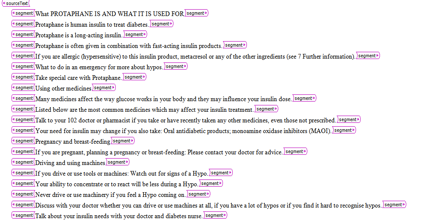
\includegraphics[width=\textwidth]{figures/Sarto8.png}
 \caption{Static scenes with evenly balanced primary and secondary areas (Joining the Dots, UK 2012)}
 \label{fig:}
\end{figure} 

\begin{figure}
 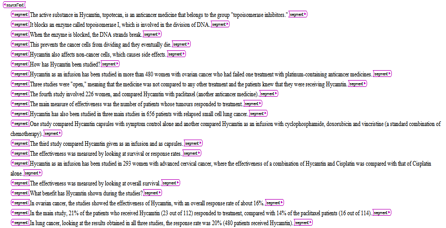
\includegraphics[width=\textwidth]{figures/Sarto9.png}
 \caption{Static scenes with evenly balanced primary and secondary areas (Joining the Dots, UK 2012)}
 \label{fig:}
\end{figure} 
 



\subsection*{Abbreviations}
\subsection*{Acknowledgements}

\printbibliography[heading=subbibliography,notkeyword=this]

\end{document}